\documentclass[]{scrartcl}


\usepackage[english]{babel}
\usepackage{euscript}
\usepackage[utf8]{inputenc}
\usepackage[ruled,vlined]{algorithm2e}

\usepackage{graphics}

\usepackage[dvips]{graphicx}

\pagestyle{headings} \makeatletter

\usepackage{verbatim}

\usepackage{pictexwd,dcpic}


% Redefine the quotient
\def\quotient#1#2{%
    \raise1ex\hbox{$#1$}\Big/\lower1ex\hbox{$#2$}%
}

\usepackage{makeidx}
\usepackage{eurosym}
\usepackage{amsfonts}
\usepackage{latexsym}
\usepackage{makeidx}
\usepackage{amsmath}
\usepackage{amsthm}
\usepackage{amscd}
\usepackage{comment}
\usepackage{enumerate}
\usepackage{mathrsfs}
\usepackage[all]{xy}

\DeclareMathOperator*{\argmax}{arg\,max}
\DeclareMathOperator*{\argmin}{arg\,min}

\usepackage{url}
\usepackage[colorlinks=true, a4paper=true, pdfstartview=FitV,
linkcolor=blue, citecolor=blue, urlcolor=blue]{hyperref}


\newtheorem{theorem}{Theorem}[section]
\newtheorem{corollary}{Corollary}[theorem]
\newtheorem{lemma}[theorem]{Lemma}

\theoremstyle{definition}
\newtheorem{definition}{Definition}[section]

%opening
\title{Bourbaki vs Pragmatism \\ A methodological comparison through the multi-armed bandits problem \\
DRAFT}
\author{Sebastiano Ferraris\footnote{sebastiano.ferraris@gmail.com}}

\begin{document}

\maketitle

% ------------------------------------------------- %
\begin{abstract}
In these pages we introduce the well known multi-armed bandits problem and we propose a solution with two different pedagogical approaches that we titled Bourbachist and pragmatic. The Bourbakist way is concerned with the mathematical foundation upon which a formal solution is derived in the shape of an axiomatic structure. In contrast, the pragmatic approach aims at finding the best algorithmic solution, reducing the mathematical formalisms to the bare minimum.
The article ends with a critical note, underlying the advantages and disadvantages of each method. \\

\noindent
If you came across this article when searching for an introduction to the multi-armed bandit problem, and not a methodological comparison, you can ignore section~\ref{se:bourbaki_perspective}. The code to create the figures and run a range of algorithms to solve the problem can be found at \href{https://github.com/SebastianoF/multi-armed-bandits-testbed}{https://github.com/SebastianoF/multi-armed-bandits-testbed}.
\end{abstract}


% ------------------------------------------------- %
\section{Multi-armed bandits problem}
\label{se:intro}
You have to repeatedly choose between $K$ different possibilities, all choices cost the same, though each may or may not provide you with a cash reward. The reward is drawn from a probability distribution, \emph{unknown} and different fro every choice.

The problem of finding a strategy to maximise the reward in this setting is called multi-armed bandits (MAB) after the situation of playing repeatedly at a row of $K$ slot machines (or single-armed bandit, as they have been called). If you have an initial amount of money of $\$1000$ and a costs of $\$1$ for each draw, than you have $1000$ attempts to balance an exploration phase when estimating the unknown distributions of each arm, with an exploitation phase, when the acquired knowledge is used for a gain the highest reward\footnote{Thompson~\cite{thompson1933likelihood} provides an early approach where the two arms are two medical treatments, Bellman~\cite{bellman1956problem} where the problem is formulated in a Bayesian perspective for two arms, and the more recent Sutton~\cite{sutton2018reinforcement}, chapter~1, where the problem introduces reinforcement learning.}.

The MAB problem can be generalised to clinical or pre-clinical trials, control engineering, mechanical and software testing, stock market investments, behavioural modelling, dynamic pricing, and many more\footnote{A survey with a list of applications of the main algorithms solving the MAB problem is proposed by Bouneffouf~\cite{bf2019survey}.}.

Goal of these pages is to introduce the problem and to provide a solution with two different methodologies:
\begin{itemize}
    \item[$\circ$] \emph{Bourbakist.} This approach, named after the collective pseudonym of the group of French mathematicians who have developed it in 1934. The initial goal of Bourbaki was to re-write one of the most widely used analysis textbook of the time, the Goursat’s \emph{Cours d'analyse mathématique}, that was considered inadequate as some counterexamples had been overlooked\footnote{A brief history of the Bourbaki and its impact in France and the rest of the world was proposed by Marmier~\cite{marmier2014idea}.}. To reach this goal and to aim at extending the possible generalisations of the problem, while keeping at the same time possible counterexamples under control also in other branches of mathematics, Bourbaki favours an axiomatic foundation based on set theory. One of the main feature characterizing this pedagogical style is that exercises, examples and the history motivating the given problem are omitted, to leave space only to the axiomatic structure.
    \item[$\circ$] \emph{Pragmatic.} In contrast with the Bourbachist approach, the pragmatic approach reduces the formalisation to its bare minimum, and it orient the effort of the reader into finding a solution of a problem, rather than the creation of a generalisable formal theory.
\end{itemize}
The MAB presented in this section, is formalised \emph{à la Bourbaki} in the next one, and presented in the pragmatic way in section~\ref{se:pragmatic_perspective}.

% ------------------------------------------------- %

\section{A Bourbakist introduction}
\label{se:bourbaki_perspective}

\begin{definition}
    Let $(\Omega, \mathcal{A})$ be a $\sigma$-algebra defined as a non-empty set $\Omega$ paired with a subset of its power set $\mathcal{A}$, containing the empty set and closed under numerable union and complement set. Let this be called \emph{action space}. Let $\mathcal{I}_{K} = \{1,2, \dots , K\} \subset \mathbb{N}$ be a set of indexes whose generic element $k$ is called \emph{arm}, by convention. Let $\mathcal{I}_{T} = \{1,2, \dots , T\} \subset \mathbb{N}$ be another set whose elements are called, again conventionally, \emph{time}. Let $\mathbb{R}_{+}$ be the positive real axis including the zero.
\end{definition}

The relationship between the above defined elements are given by a function $A$ defined as:
\begin{align*}
    A : \mathcal{I}_T \times \mathcal{A} &\longrightarrow \mathcal{I}_K \\
        (t, \omega) &\longmapsto A(t, \omega) = A_t(\omega)
\end{align*}
and by a function $R$, defined as:
\begin{align*}
\mathcal{R} : \mathcal{I}_T \times \mathcal{A} &\longrightarrow \mathbb{R}_{+} \\
(t, \omega) &\longmapsto R(t, \omega) = \mathcal{R}_t(\omega)
\end{align*}
Let the former be called \emph{action} and the latter be called \emph{reward}. Let
\begin{align*}
R : \mathcal{I}_T \times \mathcal{I}_K &\longrightarrow \mathbb{R}_{+} \\
(t, \omega) &\longmapsto R(t, k) = R_t(k)
\end{align*}
be another function, defined as the only possible function making the diagram below commutative:

\[
\begindc{\commdiag}[20]

% --- nodes:

% below
\obj(0,30)[R]{$ \mathbb{R}_{+} $}

% above
\obj(0,60)[Ik]{$ \mathcal{I}_K $}
\obj(-40,60)[A]{$ \mathcal{A} $}

% --- arrrows

% ortho
\mor{Ik}{R}{$R_{t}$}
\mor{A}{Ik}{$A_t$}

%  oblique
\mor{A}{R}{$\mathcal{R}_t$}

\enddc
\]
%
For each $t \in \mathcal{I}$. Let $R_t$ be called again \emph{reward}, and the difference between $\mathcal{R}$ and $R$ will be clear from the context.\\
We observe that $\mathcal{R}$ maps the events of the $\sigma$-algebra, while $R$ maps the corresponding indexes. This is an analogous of the definition of probability respect to the one of random variable and probability density function, for when the real axis is restricted to $[0,1]\subset\mathbb{R}$.

Now consider
\begin{align*}
    \mathcal{Q} : \mathcal{I}_T \times \mathcal{A} &\longrightarrow \mathbb{R}_{+} \\
        (t, \omega) &\longmapsto \mathcal{Q}(t, \omega) = \mathcal{Q}_t(\omega)
\end{align*}
the \emph{estimated reward of the action $\omega$ up to time $t$}, for $\omega = A_t^{-1}(k)$ for a fixed $k\in \mathcal{I}_K$, with the corresponding function $Q: \mathcal{I}_T \times \mathcal{I}_K \rightarrow \mathbb{R}$. It follows that $\mathcal{Q}$ is defined as an application of the mean value in a Lebesgue space over $(\Omega, \mathcal{A})$, that is now a Borel $\sigma$-algebra\footnote{
    For a foundational perspective, see Bourbaki~\cite{bourbaki2004integration}.
} as:

\begin{align}\label{def:mathcalQt}
\mathcal{Q}_t(\omega) = \mathbb{E} \left[ R_{\tau}(k)\mid k = A_{\tau}(\omega), \forall \tau \in \mathcal{I}_t \right]
\qquad
\omega \in \mathcal{A}
\qquad
t \in \mathcal{I}_T
\end{align}
and therefore
\begin{align}\label{def:Qt}
Q_t(k) = \mathbb{E} \left[ \mathcal{R}_{\tau}(\omega)\mid \omega = A_{\tau}^{-1}(k), \forall \tau \in \mathcal{I}_t \right]
\qquad
t \in \mathcal{I}_T
\qquad
k \in \mathcal{I}_K
\end{align}
As $\mathcal{R}$ and $R$ did, also $\mathcal{Q}$ and $Q$ satisfies the commutativity of a diagram analogous to the one shown above. The notation can be simplified for brevity\footnote{
    The simplified notation is often the only notation appearing in engineering textbooks (e.g. Sutton~\cite{sutton2018reinforcement}), although this would not allow the reader to understand the subtle formalisation of assigning to an event $\omega$ its index $k$. More tragically the simplified notation makes most of the concepts introduced so far pedantic and irrelevant.
} to:
\begin{align}\label{def:mathcalQt_simple}
Q_t(k) = \mathbb{E} \left[ R_{t}(k) \mid A_{t} = k \right]
\end{align}
where the mean value is for all the time indexes up to $t$ and where the domain values of $A_t$ is clear from the context.

\begin{definition}
    Let the \emph{total reward} $Q_{\infty}: \mathcal{I}_K \rightarrow \mathbb{R}$ be the function
    \begin{align}\label{def:mathcalQinf}
    Q_{\infty}(k) = \mathbb{E} \left[ \mathcal{Q}_{t}(\omega) \mid \omega = A^{-1}_{t}(k), \forall t \in \mathcal{I}_T \right]
    \qquad
    k \in \mathcal{I}_K
    \end{align}
    or with the simplified notation as:
    \begin{align}\label{def:mathcalQinf_simple}
    Q_{\infty}(k) = \mathbb{E} \left[ R_{t}(k) \mid A_{t} = k \right]
    \end{align}
\end{definition}

So far we have been considering the reward and the total reward for a fixed choice of $k$. We can vary $k\in \mathcal{I}_K$ in function of the time index. So let $\mathbf{k}$ an element of
\begin{align*}
\mathcal{I}_K^T = \underbrace{\mathcal{I}_K\times \mathcal{I}_K \times \dots \times \mathcal{I}_K}_{T\text{-times}}
\end{align*}
or equivalently a function from $\mathcal{I}_T$ to $\mathcal{I}_K$.
Definitions \ref{def:mathcalQt} and \ref{def:mathcalQt_simple} are so generalised to $Q_t:\mathcal{I}_K^T \rightarrow \mathbb{R}$ for $t\in\mathcal{I}_{\leq T}$, having defined $\mathcal{I}_{\leq T}$ any interval of positive integers between $1$ and $T$, and
\begin{align*}
Q_t(\mathbf{k}) = \mathbb{E} \left[ \mathcal{R}_{\tau}(\omega)
\mid
\omega = A^{-1}_{\tau}(\mathbf{k}_{\tau}), \forall \tau \in \mathcal{I}_t \right]
\qquad
\mathbf{k} \in \mathcal{I}_K^T
\qquad
t \in \mathcal{I}_T
\end{align*}
and therefore
\begin{align*}
Q_{\infty}(\mathbf{k}) = \mathbb{E} \left[ \mathcal{R}_{t}(\omega)
\mid
\omega = A^{-1}_{t}(\mathbf{k}_{t}),  \forall t \in \mathcal{I}_T \right]
\qquad
\mathbf{k} \in \mathcal{I}_K^T
\end{align*}
The mean value computed with a Lebesgue measure, over the Borel space generated as the sets of images
\footnote{
    We consider the definition under the accordance with the axiom of choice as in the ZFC axiomatic set theory, in order to avoid \emph{virages dangereux}. See also Bourbaki~\cite{bourbaki2004theory} and \cite{takeuti1982classes}.
} $\mathcal{R}_t(\omega)$ for all $\omega \in \mathcal{A}$ can be reformulated as:
\begin{align*}
Q_t(\mathbf{k})
=
\frac
{\sum_{\tau=1}^{t} R_{\tau}(\mathbf{k}_{\tau}) \mathbf{1}_{A_\tau = \mathbf{k}_{\tau}}}
{\sum_{\tau=1}^{t} \mathbf{1}_{A_\tau = \mathbf{k}_{\tau}}}
\end{align*}
where $\mathbf{1}_{A_\tau = \mathbf{k}_{\tau}}$ equals to $1$ for when the event $\omega$ corresponding to $\mathbf{k}_{\tau}$ is mapped exactly to $\mathbf{k}_{\tau}$ through $A_t$, and $0$ for any other event.
Extending the time indexes up to infinity, and to justify the notation introduced above, where we used $\infty$ for a finite case, we have the following theorem:
\begin{theorem}\label{th:bourbaki}
Given a ring of infinite cardinality to which the time index $t$ belongs, and an Hilbert module\footnote{An algebraic structure generalising Hilbert vector spaces over the now introduced ring of time indexes. See for example \cite{bourbaki1987topological}.} to which the vector $\mathbf{k}$ belongs, it follows that
\begin{align*}
Q_{\infty}(\mathbf{k}) = \lim_{T \rightarrow \infty} Q_{T}(\mathbf{k})
\end{align*}
\end{theorem}
\begin{proof}
    Direct consequence of the definition of $Q_{\infty}$ generalised to the theorem hypothesis' extended structures.
\end{proof}

We now consider the value $\hat{k}$ that satisfies
\begin{align*}
\hat{k} = \argmax_{k \in \mathcal{I}_K} Q_t(k)
\qquad
\forall t \in \mathcal{I}_T
\end{align*}
for a constant value for each time index, as in the definition of $Q_t$ given in~\ref{def:Qt}.
If we consider the possibility of varying the chosen arm $k$ across time, and so if we are allowed to compare different images of the function $A_t$ then $\hat{\mathbf{k}}$ is defined as
\begin{align}\label{eq:bourbaki_solution}
\hat{\mathbf{k}}
=
\argmax_{\mathbf{k} \in \mathcal{I}_K^{T}} Q_t(\mathbf{k})
\qquad
\forall t \in \mathcal{I}_T
\end{align}
Under the light of theorem~\ref{th:bourbaki}, and with the given definitions, we can now call the so defined vector $\hat{\mathbf{k}}$ the \emph{solution of the generalised multi-armed bandits problem}.

% ------------------------------------------------- %
\section{A Pragmatic (non-Bourbakist) introduction}
\label{se:pragmatic_perspective}

\subsection*{Creating a Benchmark}

To have a ground truth of the multi-armed bandit problem where to test a range of algorithms and parameters, we consider a benchmark dataset where the distribution of each arm is known.
In the particular case we are dealing with, we assume each arm normally distributed, with mean sampled from a uniform distributions in the interval $[-3, 3]$ and the standard deviation sampled again from a uniform distribution on the interval $[2, 3]$. A representation of these distribution is plotted in
figure~\ref{fig:volin_plot}.

If the studied case is modelled with a different distribution, what is said in this section is still applicable simply adapting this benchmark to the intended distribution.

\begin{figure}[h]
    \hspace{-1.5cm}
    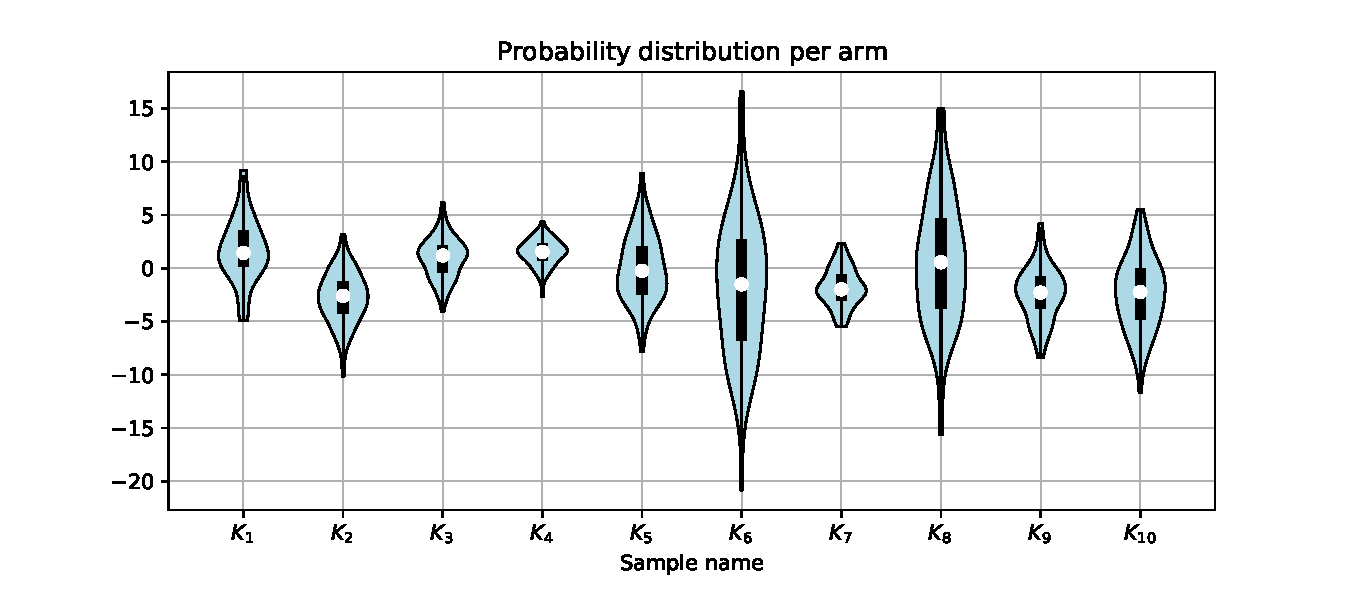
\includegraphics[width=18cm]{figures/initial_distributions.pdf}
    \caption{The distributions of the random reward for each arm $K$, unknown to the player, are sampled from normal distributions, with mean uniformly sampled in the interval $[-3, 3]$ and standard deviation in the interval $[1, 2]$.}
    \label{fig:volin_plot}
\end{figure}

\subsection*{Encoding the problem}
For the player, the MAB is a reward for a given arm index $k$, pulled at time $t$. We encode the rewards in a $T\times K$ \emph{reward matrix} $q$. In our example $T=1000$ is the time we will be pulling an arm and $K=10$ is the number of arms. The element $q_{t, k}$ represents the reward collected for having pulled the arm $k$ at the time-point $t$. As we can pull only one arm at a time, there is only one known value for each column of the matrix. All the other values are initialised to nan.

We also consider the non-stationary case, where the means and the standard deviations of the arms distributions represented in figure~\ref{fig:volin_plot} are not constant over time. We encode  the MAB with the matrices $\mu$ and $\sigma$ having shape $T_{\text{arm}} \times K$ and providing the mean and standard deviation of the distribution of the arm $k$ at time $t$.

The rewards can be accumulated for more or less numerous time points than $T_{\text{arm}}$, as the distributions of the arms can repeat. If $T_{\text{arm}}=1$ then the problem is stationary, and if $T=30$ and $T_{\text{arm}}=15$ then each arm $k$ will be looping over its parameters $\mu_{:, k}$ and $\sigma_{:, k}$ twice, according to:
\begin{align*}
q_{t, k}
=
\text{norm}\left(\mu({t~\text{mod}~T_{\text{arm}}, k}), \sigma({t~\text{mod}~T_{\text{arm}}, k})\right)
\end{align*}
where $\text{norm}(\mu, \sigma)$ is the normal distribution of location $\mu$ and scale $\sigma$ and mod is the modulo operator.

\subsection*{$\epsilon$-greedy algorithms}

The family of $\epsilon$-greedy algorithms to solve the MAB problem is based on the idea that if your bad luck is consistent, probably it is not just bad luck. The multi armed bandit is approached alternating between a phase of exploration (proportional to $\epsilon$ times), and a phase of exploitation (proportional to $1 - \epsilon$ times). In the first phase, the player acquires informations about the structure of the problem regardless the immediate gain. In the second phase the informations gained are used to maximize the reward\footnote{
    An accurate historical introduction of this family of algorithms can be found at the end of chapter~1 of~\cite{sutton2018reinforcement}.
}.

The basic version of the $\epsilon$-greedy algorithm (or \emph{naive $\epsilon$-greedy}), selects a random arm when exploring and the arm that had obtained the best reward so far when exploiting. This can happen after an initial phase of pure exploration, where only random arms are pulled. An example of the application of this algorithm is shown in figure~\ref{fig:step_32}.

A more sophisticated version that the naive $\epsilon$-greedy is the \emph{best reward $\epsilon$-greedy}. In this case, instead of selecting any random arm in the exploration phase, we weight the random selection using the rewards obtained so far, and excluding the arm with the highest reward. With this strategy we will be more likely to explore the arms that have provided good rewards in the past, and to refrain from spending money over an arm that have never provided a reward.

A third algorithm is the \emph{least explored $\epsilon$-greedy}. In the exploratory phase of this algorithm we increase the probability of falling over the least explored arms, instead of the one providing the highest reward. This method and the previous one are both aimed at preventing from getting stuck in a local minima, or an arm that is good enough to have a gain, but that is not the optimal one.

\begin{figure}[h]
    \hspace{-1cm}
    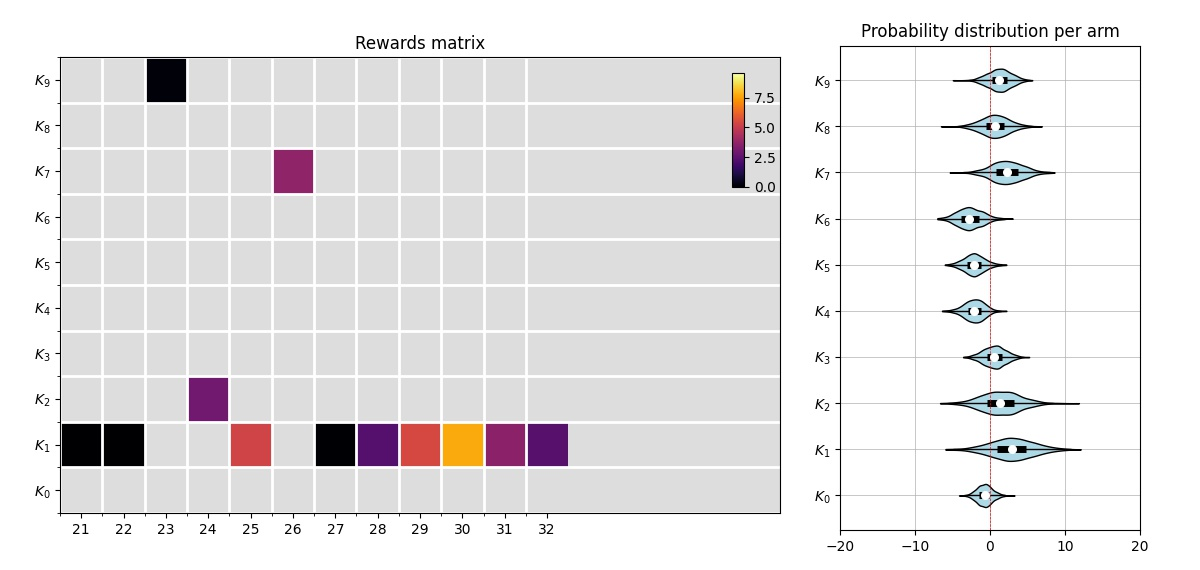
\includegraphics[width=17cm]{figures/step_32.jpg}
    \caption{The reward matrix after $32$ steps of a \emph{naive} $\epsilon$-greedy algorithm. We can see that step $23$, $24$ and $26$ are explorations in a row of exploitation of the arm $7$ that so far had produced the highest reward. To the grey colour corresponds the nan value used to initialise the reward matrix. In this instance, the reward is clipped at zero, as the loss of money is only the cost of pulling an arm at each time-point.}
    \label{fig:step_32}
\end{figure}

The fourth algorithm here presented is the \emph{upper confidence bound $\epsilon$-greedy algorithm} \cite{sutton2018reinforcement}, where the estimated optimal arm at time $t$, is given by
\begin{align}\label{eq:upper_confidence_formula}
\hat{k}_t = \argmax_{k} \left[ \hat{\mu}(k) + \lambda \sqrt{ \frac{\ln(t)}{ N_{t}(k) }  } ~\right]
\end{align}
where $N_{t}(k)$ is the number of times the armed $k$ had been pulled up to the time $t$, which can be easily computed from $q$. The regularisation term weights the uncertainty in the estimate, correcting for underestimation of the estimated mean.

Note the player will receive $0$ when the sampled reward is below $0$. This means that the estimated mean does not correspond to the one of the original distribution, though the result will be conservative in having an observed average close to zero for distribution whose mean is below the zero. The reader should resist the temptation of estimating the arm using the mode instead of the average in equation~\ref{eq:upper_confidence_formula}. In fact if the standard deviations are very different across arms, a very inconvenient arm may be identified as the optimal one.

The performance of these algorithms are all depending upon problem distribution, and the optimal one should be found empirically via simulation. Providing a benchmarking for a general case would not be useful here. What provides the constraints to make the case less general, is based on the instance of the problem to which the algorithms are applied. A platform where to make further experiments is open-sourced at~\href{https://github.com/SebastianoF/multi-armed-bandits-testbed}{https://github.com/SebastianoF/multi-armed-bandits-testbed}.


% ------------------------------------------------- %
\section{Comparing the two methodological approaches}
\label{se:outro}

In this article, we considered the example of the multi-armed bandit problem to show two different methodological approaches towards its solution.

The Bourbaki presentation in section~\ref{se:bourbaki_perspective} is based on an axiomatisation of the problem and it evolves from a functional and set-theoretical perspective. It focuses on the symbolism, and according to the Bourbachist tradition, it provides no examples or algorithms, as the only connecting point between the theory and the given problem is the axsiomatic setting.

Assuming that this approach is correct (excluding typos) and coherent (excluding Goedel\footnote{
    To this regard, in the article \emph{the ignorance of Bourbaki}~\cite{mathias1992ignorance}, Mathias noticed that the attempt of grounding the whole corpus of mathematics in an axiomatic sense have happened after, and in a conscious effort of ignoring the Goedel incompleteness theorems.
}), it is easy to see that it had the effect of turning a relatively simple problem into a complicated maze of interrelated concepts, having mainly the consequence of pushing the reader away from the practical solution.

On the contrary, the pragmatic approach of section~\ref{se:pragmatic_perspective} shows that there is no need of taking a functional perspective and to connect it to several mechánemas to prevent counterexamples (Borel spaces, Lebsgue Measures...) developed in entirely different contexts, and no need to extend the bibliography beyond one ot two resources. Borel spaces and any element of measure theory are not just irrelevant in aiming at a solution, they are also reducing any possible creativity when facing a slightly different problem, as the variation of the unknown distributions over time. If in doubt on this point the reader is invited to continue the formalisation in this direction, to see how many pages and new definitions and diagrams are needed. We also challenge the reader to implement the code to solve the problem having only the functional and algebraic definitions at hand rather than relying on the matrix point of view.

%None of the given definitions in the Bourbaki approach had provided any hints on how to really solve the problem, in a numerical sense, as, in conformity with the Bourbaki style, no examples had been provided.

\subsection*{Other examples}

Certainly the example provided is biased by the fact that they are the best approximation of a Bourbaki approach and of a pragmatic approach that the author could attain.

To this regard there are numerous cases of practical problems, whose pragmatic approach had been overformalised in a similar fashion\footnote{
    Or \emph{assiomattisation}, as Bruno de Finetti~\cite{de2008bruno} would have said playing on the Italian word \emph{matti}, meaning crazy.
}. These are all useful examples, in particular to anyone who may believe that the author had been overzealous in writing section~\ref{se:bourbaki_perspective} to give on purpose a negative light upon this methodology.

The most notable example is the optimal transport (OT) theory. From being a pragmatic tool of solve a class of optimisation problems, it had become a $500$ pages book underpinned by a great amount of measure theory and Lebesgue spaces, perfectly irrelevant to solve any instance of an optimal transport problem, when the reader will have to face one. Comparing one of the original optimal transport theory introduction, for example the one by Hitchcock~\cite{hitchcock1941distribution}, with the formalised version by Villani~\cite{villani2003topics} it is possible to see the issue. The first one is easy to read, understand, implement and possibly extend in several directions by anyone having an high school mathematical education. The second one is a seemingly uncreated maze of unassailable interlinked concepts, requiring few years of academic studies only to grasp the first few pages, with no advantages in finding a numerical solution to the problem. %It is almost impossible to be extended in any direction that a slightly different initial problem arising from practical need may pose, and it leaves no clarification whatsoever about why this perspective should be preferred upon the one proposed 60 years before. %Not surprisingly, a recent evolution of the OT by Patel~\cite{patelalternate} is rooted in the pragmatic approach, and does not even cite the Villani formalisation.

A second notable example of the Bourbachisation is in the domain of medical image registration. Here the aim is to solve the problem of finding the non-rigid deformation or metamorphosis between anatomies. The problem originates from the anatomical studies of shapes growth by D'Arcy Thompson~\cite{d1942growth} and pragmatically extended amongst others in Modersitzki~\cite{modersitzki2004numerical}. The Bourbaki over-formalized branch can be found in works like~\cite{younes2010shapes}, where we have to wait for 12 chapters before seeing what had motivated the formal mathematical theory developed until there.
In this case too, there is no explanation of what are the advantages of the axiomatic approach respect to the pragmatic one, appeared half a century earlier.

The reader may say, for this specific case, that the pragmatic approach \cite{modersitzki2004numerical} does not use neither diffeomorphisms nor reproducing Kernel Hilbert spaces. And this is true, although it is not proved that these two mathematical devices can provide more accurate results than their pragmatic counterparts when implemented in practice. Instead it is true that they are computationally slower.


\subsection*{The Bourbaki pattern}

There are other examples in the literature where we can find a comparison between the Bourbaki / pragmatic approach, such as algebraic topology, fuzzy logic and topological data analysis. Their detachment from the practical set of problems that had them originated, had turned them into convoluted axiomatic buildings, where it is not possible to find any breakthrough result, or even practical help, in the perspective of solving the initially given problem.

It is at this point evident the existence of a pattern in the process of Bourbachisation: a problem solved by more than 50 years, and often in a very elegant and practical way, was taken under the wing of the academic axiomatisers and transformed into a list of definitions and theorems where no echo of the original problem motivating the theory can be found.

%Remarkably, also Einstein had noted that \emph{Since the mathematicians have invaded the theory of relativity, I do not understand it myself any more} \cite{schilpp1951albert}. And it is difficult to find what are the new results that the Bourbaki formalisation have added to the theory of relativity.

What is also constant in the Bourbaki pattern is that the formalised version of the practical theory adds no value to it. No new results having any practical relevance can be found in the work by Bourbaki and their followers.

There is only one notable exception to this rule that we could find. The work Mochizuki~\cite{mochizuki2012inter} is claimed to have solved the \emph{abc conjecture}. Worth of a pantomime, according to the mathematicians who had tried to read this work, \lq\lq the proof is too impenetrable to be understood\rq\rq\footnote{As statement published in Nature, Castelvecchi~\cite{castelvecchi2015biggest}.}.

\subsection*{Why is Bourbaki still around?}

%What the examples proposed in these pages intended to show, from a qualitative and empirical evaluation, is that the over-axiomatic version of a theory has several negative aspects respect to its pragmatic counterpart.

%These are: Bourbaki formalisation has an exhaustive cognitive load,increases the difficulties that a generalisation of a simple change in the initial problem setting may require. It is by no mean close to the formalisation that is required to be implemented in modern programming language. Bourbaki does not provide any additional insight and intuition over the problem that originated the theory. The reader get used to work on useless details and pedantic discussions about notations, rather than solving the problem.




These pages are not written to accuse Bourbaki. Their goal is rather to try to analyse and understand.
It is true that despite many, have express their negative view about the Bourbakist's mathematics\footnote{
    Amongst the many: Arnold~\cite{arnol1998teaching}, De Finetti~\cite{de2008bruno}, Lockhart~\cite{lockhart2009mathematician}, the already cited Mathias and its follow up~\cite{mathias1998further}, Velupillai~\cite{velupillai2012bourbaki}. And even the article by Marmier~\cite{marmier2014idea}, that sees the Bourbaki movement with enthusiasm and appreciation for their work and impact in the society, begs some questions when it says
    \lq\lq Living mathematics is being done elsewhere in the world, in connection with new problems arising from other disciplines or other human activities\rq\rq.
}, the Bourbaki approach is still widespread if not predominant across the mathematical community and also greatly valued, prized, and appreciated by academics\footnote{
    To this regard, the active reader is welcome to copy-paste section~\ref{se:bourbaki_perspective} and to extend it, in the Bourbakist style, into an article whose title could be something like \emph{The multi-armed bandits for the working mathematician}, to see how this would be received by the mathematical community.
}.

Very often, the over-axiomatization of a theory developed outside academia by scientists chasing practical problems had received several recognitions, including the Fields Medal.
Highly valued and cited uber-bourbachists works are for example Grotedniek~\cite{grothendieck2011some} and the already mentioned four volumes of Mochizuki~\cite{mochizuki2012inter}\footnote{
    It is also interesting to notice at this point the similarity between this work and the outcome of the randomized generator of maths paper at \href{https://thatsmathematics.com/mathgen/}{thatsmathematics.com/mathgen/}.
}.


Is it then really true that the Bourbachisation has no practical use? Below are itemized all the reasons that the author could find to justify the success of the Bourbaki school.

\begin{itemize}
    \item[$\circ$] \emph{The outcome of the Bourbaki approach is inaccessible to neophytes}\footnote{
        An attempt of turning an over-formalised Bourbakist theory into something accessible for the layman, can be found in Villani~\cite{villani2003livingtheorem}. Interestingly enough, it seems that the only way the author could popularize his theory was by omitting the definitions and proofs while leaving only the main mathematical formulas alongside some autobiographical events. The result is even less accessible than the original work, proving that mathematicians can also be successful surrealist artists.
    }, and it allows the existence of professors of mathematics who can not code or do not have any ability to solve any problem in practice. This seems to be the main reason that justifies the continuation of the Bourbachism, as neophytes usually are the people who have to decide where the public money goes and professors the ones who receives it.

    \item[$\circ$] \emph{The Bourbaki approach is good for the ego}. The pleasure of owning an elegant notebook filled with mathematical formulae written with a well thought after handwriting is a most sublime one. Unfortunately, after empirical evidence we can assure that this very same pleasure is a great obstacle in acquiring knowledge. The notebook owner, when facing a problem, will inevitably tend to abandon any scientific method and will bend the problem to the behold solution. To this regard, it would be interesting to measure scientifically the dopamine level of group of mathematician trying to solve a difficult problem respect to a group tweaking axioms to make the theory more abstract.

    \item[$\circ$] \emph{Bourbachism detaches completely mathematics from reality}, so it makes impossible to have any objective measurement of the quality or value of the work produced, besides the readers' opinion. This is a very unscientfic feature, and again a very useful one for whoever must defeat  more skilled competitors within the academic environment.

    The advocates of the superiority of pure mathematics\footnote{
        It is worth noticing that the academic dichotomy pure/applied maths is something that can not be found in mathematics before Bourbaki. The reader is invited to classify any of the work of Archimedes, Gauss, Euler or any other great names in the history of pre-modern mathematics as pure or applied mathematics with no ambiguities.
    } have even arrived at accusing the mathematics that have anything to do with reality of being more prone of making mistakes\footnote{
        Gros~\cite{gros2019masters} had found how even professional mathematicians can be mislead by reality. And they had leveraged on this most surprising fact, for advocating to increase the detachment. After concluding that \lq\lq [...] we can't reason in a totally abstract manner\rq\rq, instead of suggesting to take into account the reality in the mathematical practice they suggested a move towards the opposite direction: \lq\lq We have to detach ourselves from our non-mathematical intuition\rq\rq~\cite{gros2019sciencedaily}.
    }. We can be reassured by the fact that under every circumstance, the reality is adamant to persist in being what it is, and it is at this point an interesting exercise to imagine someone advocating for having medicine and engineering detached from reality.

    \item[$\circ$] \emph{The Bourbaki inspired work are more generalizable}. While this appear to be true at first glance, we claim that on the contrary a Bourbaki theory is less generalisable. Simply adding a new or different assumption to the problem settings would require to re-write almost from scratch all the axiomatic building to include the new input in a generalisable manner. The pragmatic way provides handle on the problem that are easy to be tuned or re-adapted to a slightly different one.

    \item[$\circ$] \emph{Bourbachism binds the concepts in formal structures avoiding paradoxes and counterexamples}. This is a very valid point in favour of the Bourbakist method, as the concerns of mathematics with counterexample have led to various discoveries, from Galois theory, to Fractals, and the search for counterexample is a valuable tool to have a better understanding when exploring the limits of mathematical knowledge\footnote{
        For example Procesi~\cite{procesi1977elementi}, Mandelbrot~\cite{mandelbrot1983fractal} and Gelbaum~\cite{gelbaum2003counterexamples}.
    }. Although, the problem of the Bourbaki approach is the over-concern with counterexamples originating from theoretical considerations not related in any way to the sought solution. In section~\ref{se:bourbaki_perspective} we attained an algorithm that solves the problem, having never faced pathological counterexamples despite not relying on $\sigma$-algebras, Borel spaces, Lebesgue measures or even without explicit use of functions. What we came across were only some practical malices of the craft that are never learned by whoever is limiting themselves to the Bourbaki presentation of the problem.

\end{itemize}

About this last point in particular, there is an (in)famous case where over-concerned researchers had been mislead by a misquoted counterexamples: the medical imaging paper by Lorenzi~\cite{lorenzi2013geodesics} claims that there is no bijective correspondence between the space of the tangent vector fields and the one of their integral curves. This claim is made after citing a very peculiar counterexample found in one of the Milnor research papers, involving the tangent space of the circle.

Interestingly enough the conditions for the counterexample to happen are never met in the applications presented in the paper dealing with $\mathbb{R}^3$, whose tangent space is $\mathbb{R}^3$ itself and the bijective correspondence is guaranteed by the theorem of existence and uniqueness for ODEs.


% ------------------------------------------------- %
\section{Conclusion}

If we wanted to divide the mathematical approaches into two, we would consider the Pythagorean and the Archimedean schools of thought. The Pythagorean school, influenced by the ancient Egyptian and Persian mathematics, considers the mathematical practice as a tool to investigate and measure the reality and to find the connections between apparently distinct elements through abstraction and generalisation\footnote{
    As for example astronomy, music and architecture~\cite{robins1995mathematics}, \cite{boyer2011history}.
}
. The Archimedean vision sees mathematics as a tool to solve very practical problems, approaching them with heuristic, algorithms and even adhoceries\footnote{
    An example of this approach is the proof of the formula for the parabolic segment's area by Archimede~\cite{boyer2011history} and \cite{strogatz2019infinite}.
}. To neither the Pythagorean nor the Archimedean belongs the dichotomy between pure and applied mathematics, as there is no concept of \emph{pure} in the sense of detached from the reality, being the reality always the centre of the investigation.

Neither the Bourbachist vision does belong to these two mathematical schools: it is neither oriented towards finding hidden connections between apparently separated phenomenon, nor towards solving practical problems. The manipulation of abstract structure arising from the need of finding a proof that is general enough, in the Bourbachisation had shifted its aim: from looking at the problem it had started wandering around the creation of abstract buildings where anything that is coherent with the initial axioms can be added, even if it does not solve problems or shows hidden connections. The unavoidable contraindication si that the abstract building are destined at becoming labyrinths without a centre.

Only from this point onwards, the subdivision between pure and applied mathematics had been required, as a line draw between mathematical practice (either of Pythagorean or Archimedean school) and the axiomatisation.

The comparison proposed in this paper, through the multi-armed bandit problem, aims at providing an example between the pure and applied approach towards the same problem and collects a list of similar cases in literature, where the Bourbachism had shifted the focus from the problem to the axioms, and where the reader can only find an over-formalised list of definitions and theorems of no use outside academic discussions.

When the pragmatic perspective is applied to the same problem, an algorithmic solution can be quickly explained, and the explanation is enough to provide the guideline to implement and test a range of algorithms. All this without calling into play Borel or Lebesgue, as done in the counterpart.

%
%
% in achieving a possible solution of a problem, and how choosing the wrong approach, would end up in never reaching anything useful. The paper shows the over-formalised approach first, and the pragmatic approach in the subsequent section.
%
%
%In the discussion we challenged the usefulness of the Bourbaki approach outside its circle of academics. The Bourbaki generalisations are not practical and the counterexamples that are excluded by the overformalisation do not arise in practice. the author also implies that the mindset of the Bourbaki educated student can even obstaculate the pathway leading to a solution of a practical problem.
%
%Despite the author is convinced that students of the generations to come will be obliged to learn the Bourbaki sophistications to get a degree, and to unlearn them as quickly as possible to be of any use to the non-academic society, this paper hopes to show that the Bourbaki method is around for academic reasons, and it is not what mathematical practice is about or should be. %which is the application of the scientific method to understand the reality and to find the best algorithm that solves a given problem.


\bibliography{biblio}
\bibliographystyle{alpha}


\end{document}
